\documentclass[11pt,letterpaper]{article}

\usepackage[margin=0.9in]{geometry}
\usepackage{amsmath,amssymb}
\usepackage{graphicx}
\usepackage{booktabs}
\usepackage{float}
\usepackage{caption}
\usepackage{enumitem}
\usepackage[colorlinks=true,linkcolor=black,urlcolor=blue]{hyperref}

\graphicspath{{figures/}}
\captionsetup{font=small,labelfont=bf}

\newcommand{\sreach}{\mathcal{S}_{\mathrm{reach}}}
\newcommand{\QVI}{Q^*_{\mathrm{VI}}}
\newcommand{\piVI}{\pi^*_{\mathrm{VI}}}

\title{CS 4/5789 --- Programming Project 3:\\Balloon Navigation}
\author{Alexander Braverman}
\date{October 14, 2026}

\begin{document}
\maketitle

All three methods were implemented in \texttt{DP.py}, \texttt{VI.py} and
\texttt{Qlearning.py}; \texttt{python test.py} passes every check. All
figures below were produced by
\texttt{python visualize.py --experiment all --save-dir figures} with the
default settings (seed 0). Throughout, the start state is $s_{(1,0)}$ and
the goal is $s_{(5,5)}$. Two routes to the goal matter for almost every
result:
\begin{itemize}[nosep]
  \item \textbf{Risky route (7 steps):} DOWN twice, so the rightward wind
    along the bottom row carries the balloon through two $-5$ cells to
    $(3,0)$; then UP five times, with the rightward winds at $(3,1)$ and
    $(4,2)$ pushing it into column 5. Undiscounted return
    $-5-5-1-1-1-1+20 = \mathbf{6}$.
  \item \textbf{Safe route (14 steps):} UP column 1, across the top, DOWN
    column 3 until the wind at $(3,1)$ pushes it to $(4,1)$, then UP into
    column 5 and up to the goal. Thirteen $-1$ steps then $+20$:
    undiscounted return $\mathbf{7}$.
\end{itemize}
Column 0 has no rightward wind anywhere, so a balloon that enters it can
never leave; it is a trap worth $-1$ per step forever. (It is also
unreachable from the start, so Q-learning never sees it.)

%------------------------------------------------------------------
\section*{6.1 Dynamic programming (finite horizon)}

\begin{table}[H]
\centering
\begin{tabular}{ccl}
\toprule
$H$ & $V^*_0(s_0)$ & Route from start \\
\midrule
1  & $-1$ & goal unreachable \\
3  & $-3$ & goal unreachable \\
5  & $-5$ & goal unreachable \\
7  & $6$  & risky (exactly fits) \\
9  & $6$  & risky \\
14 & $7$  & safe (first horizon it fits) \\
\bottomrule
\end{tabular}
\end{table}

\begin{figure}[H]
\centering
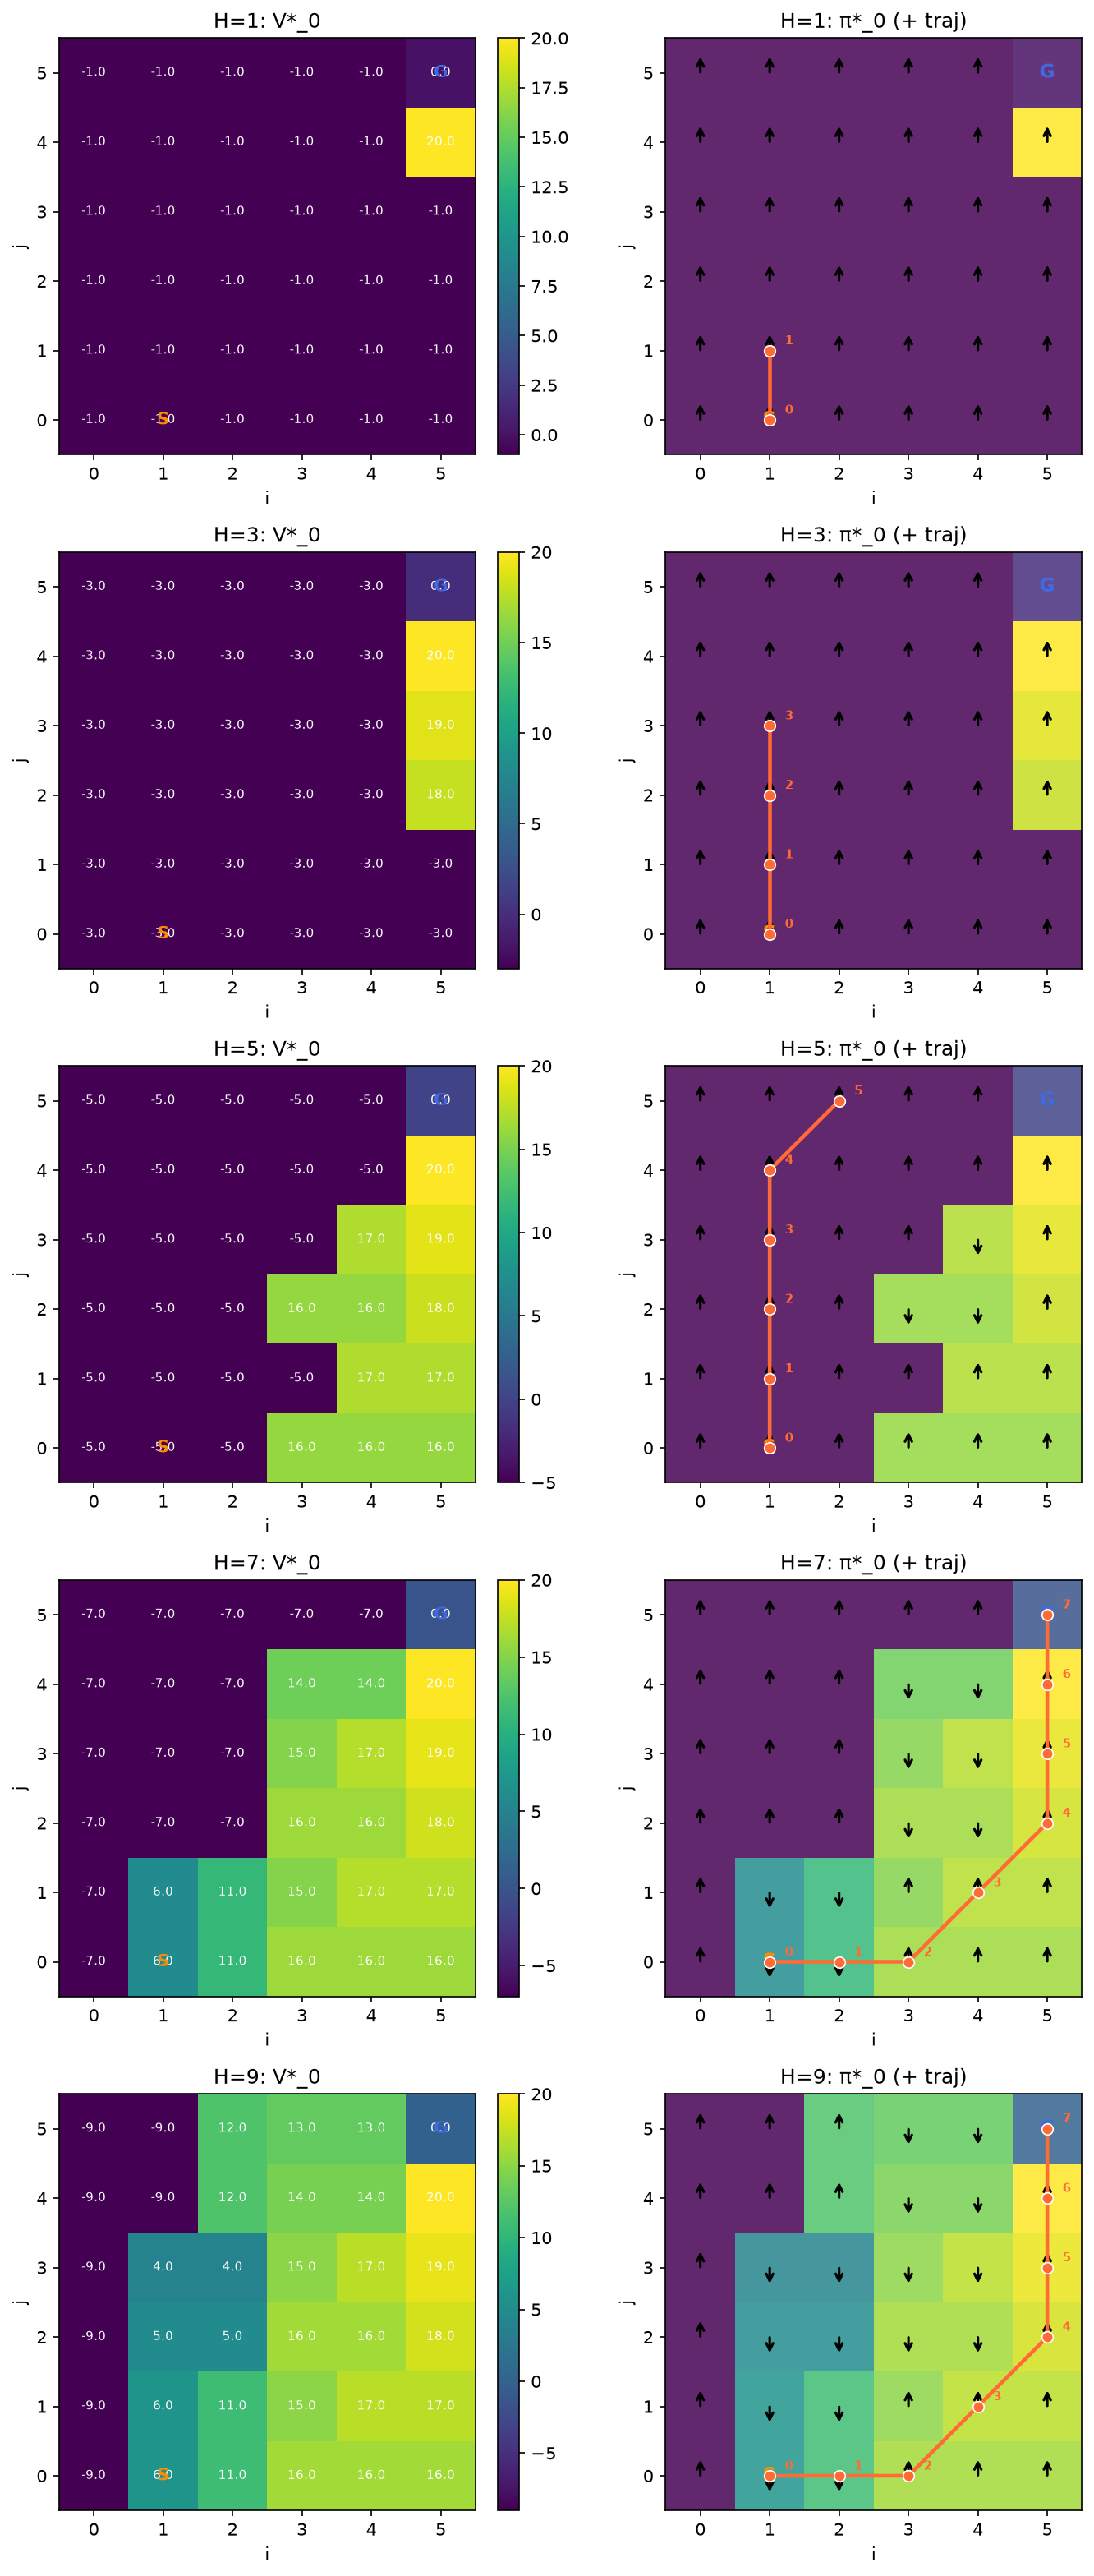
\includegraphics[height=0.82\textheight]{dp_horizon_sweep.png}
\caption{$V^*_0$ (left) and $\pi^*_0$ with the greedy trajectory from the
start (right) for $H \in \{1,3,5,7,9\}$.}
\label{fig:dp-sweep}
\end{figure}

\begin{figure}[H]
\centering
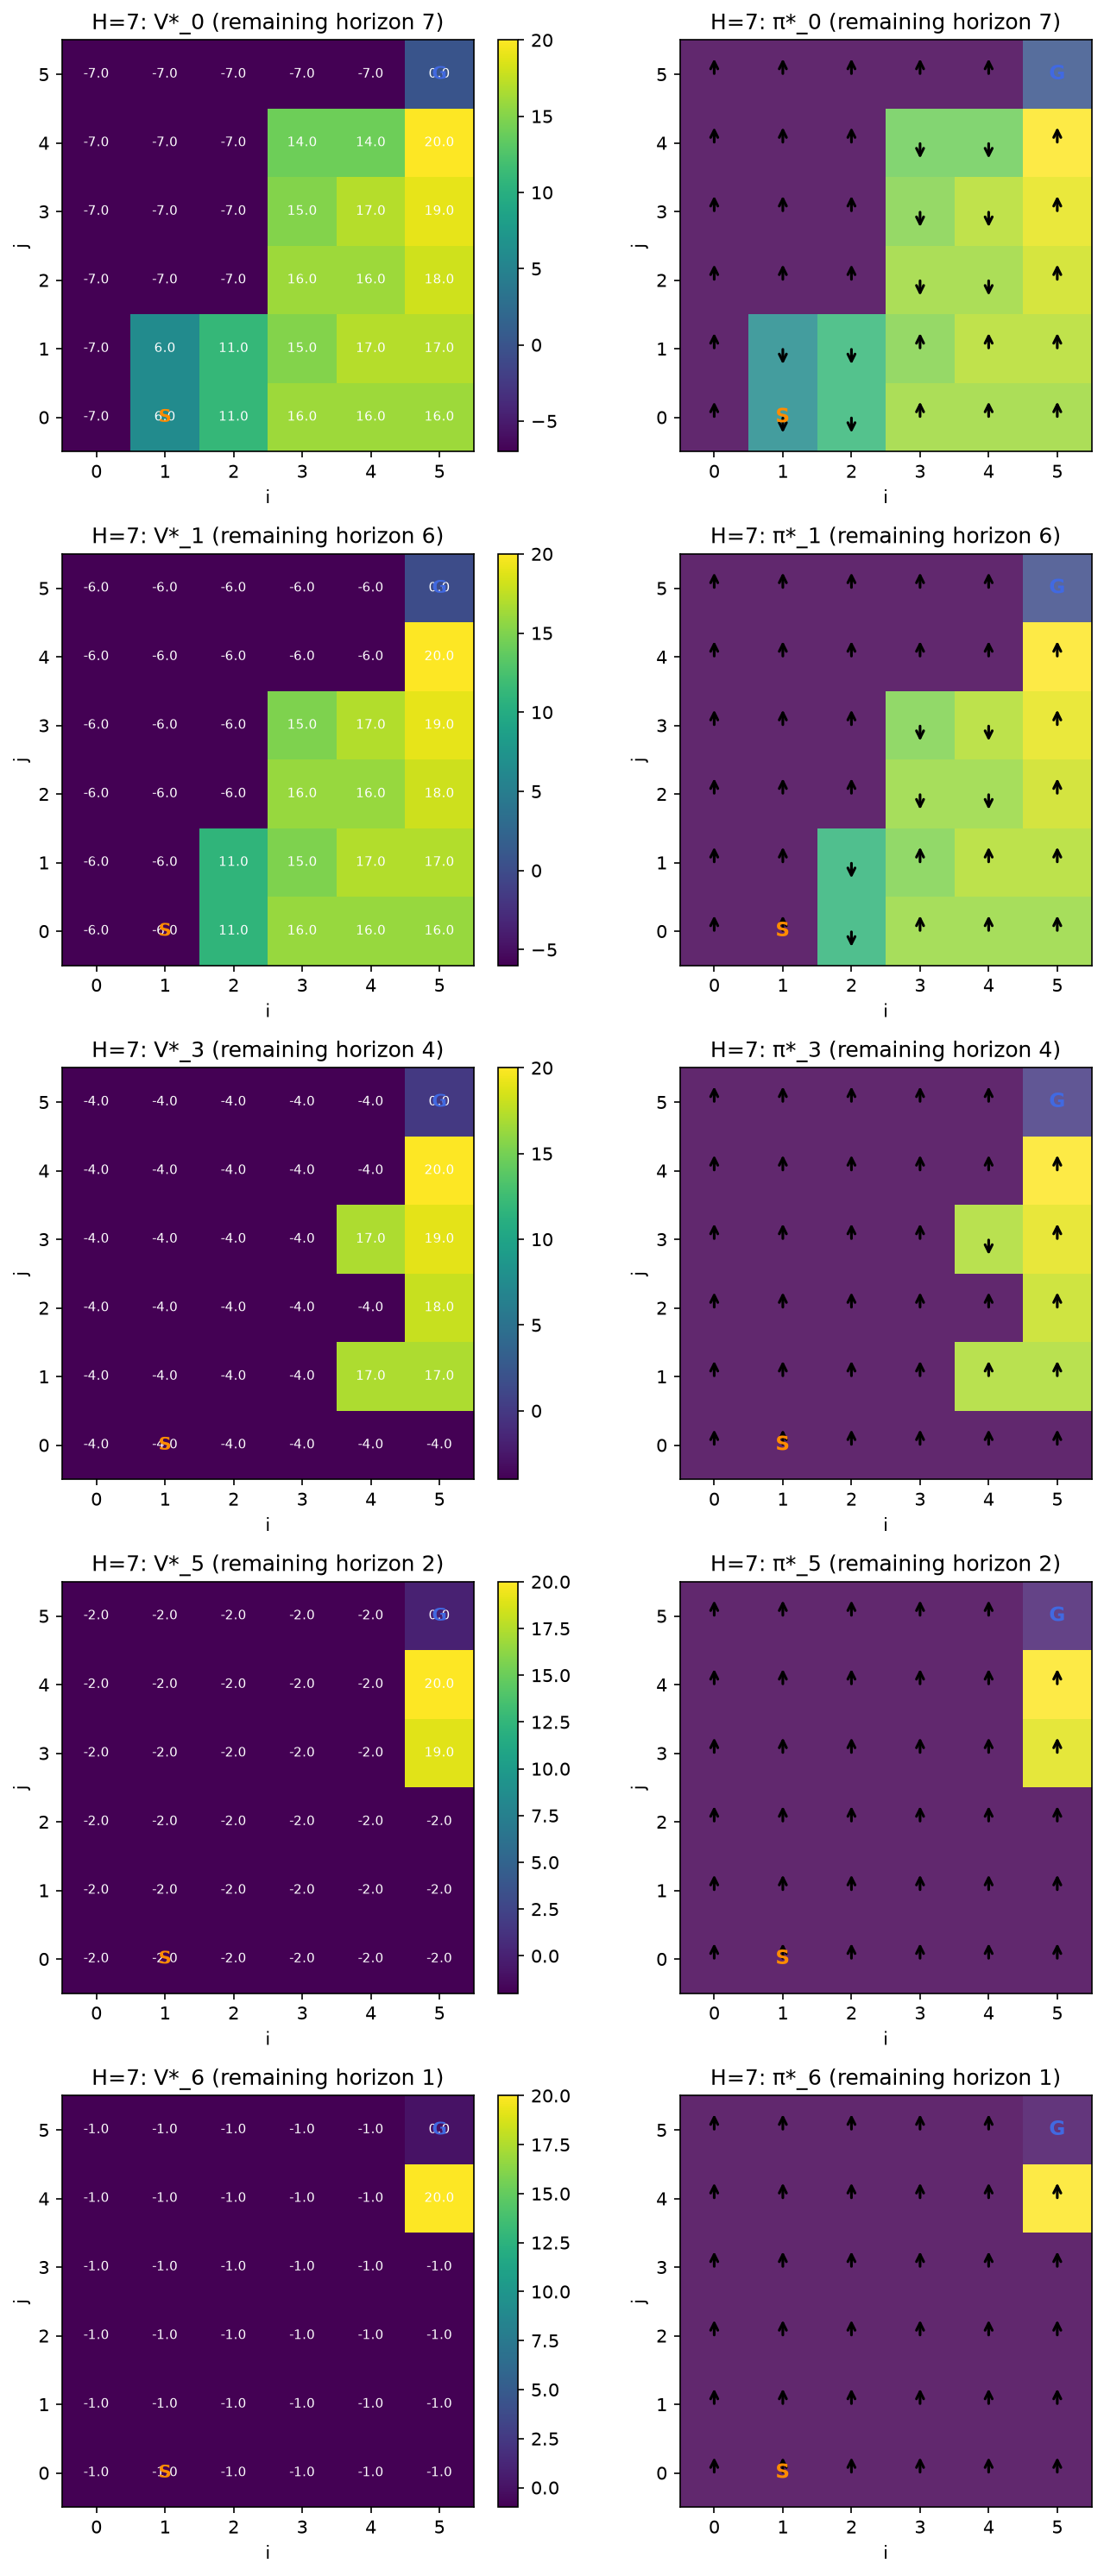
\includegraphics[height=0.82\textheight]{dp_time_slices_H7.png}
\caption{$H=7$: time slices $(V^*_t,\pi^*_t)$ for $t = 0,1,3,5,6$, i.e.\
remaining horizon $7,6,4,2,1$.}
\label{fig:dp-slices}
\end{figure}

%------------------------------------------------------------------
\section*{6.2 Value iteration (infinite horizon, discounted)}

\begin{table}[H]
\centering
\begin{tabular}{ccccl}
\toprule
$\gamma$ & Iterations to tol $=0.01$ & $V^*(s_0)$ & $V^*(\text{column } 0)$ & Route from start \\
\midrule
0.9   & 45   & $-1.66$ & $-9.9$   & risky \\
0.99  & 460  & $5.30$  & $-99.0$  & safe \\
0.999 & 4607 & $6.82$  & $-990.1$ & safe \\
\bottomrule
\end{tabular}
\end{table}

\begin{figure}[H]
\centering
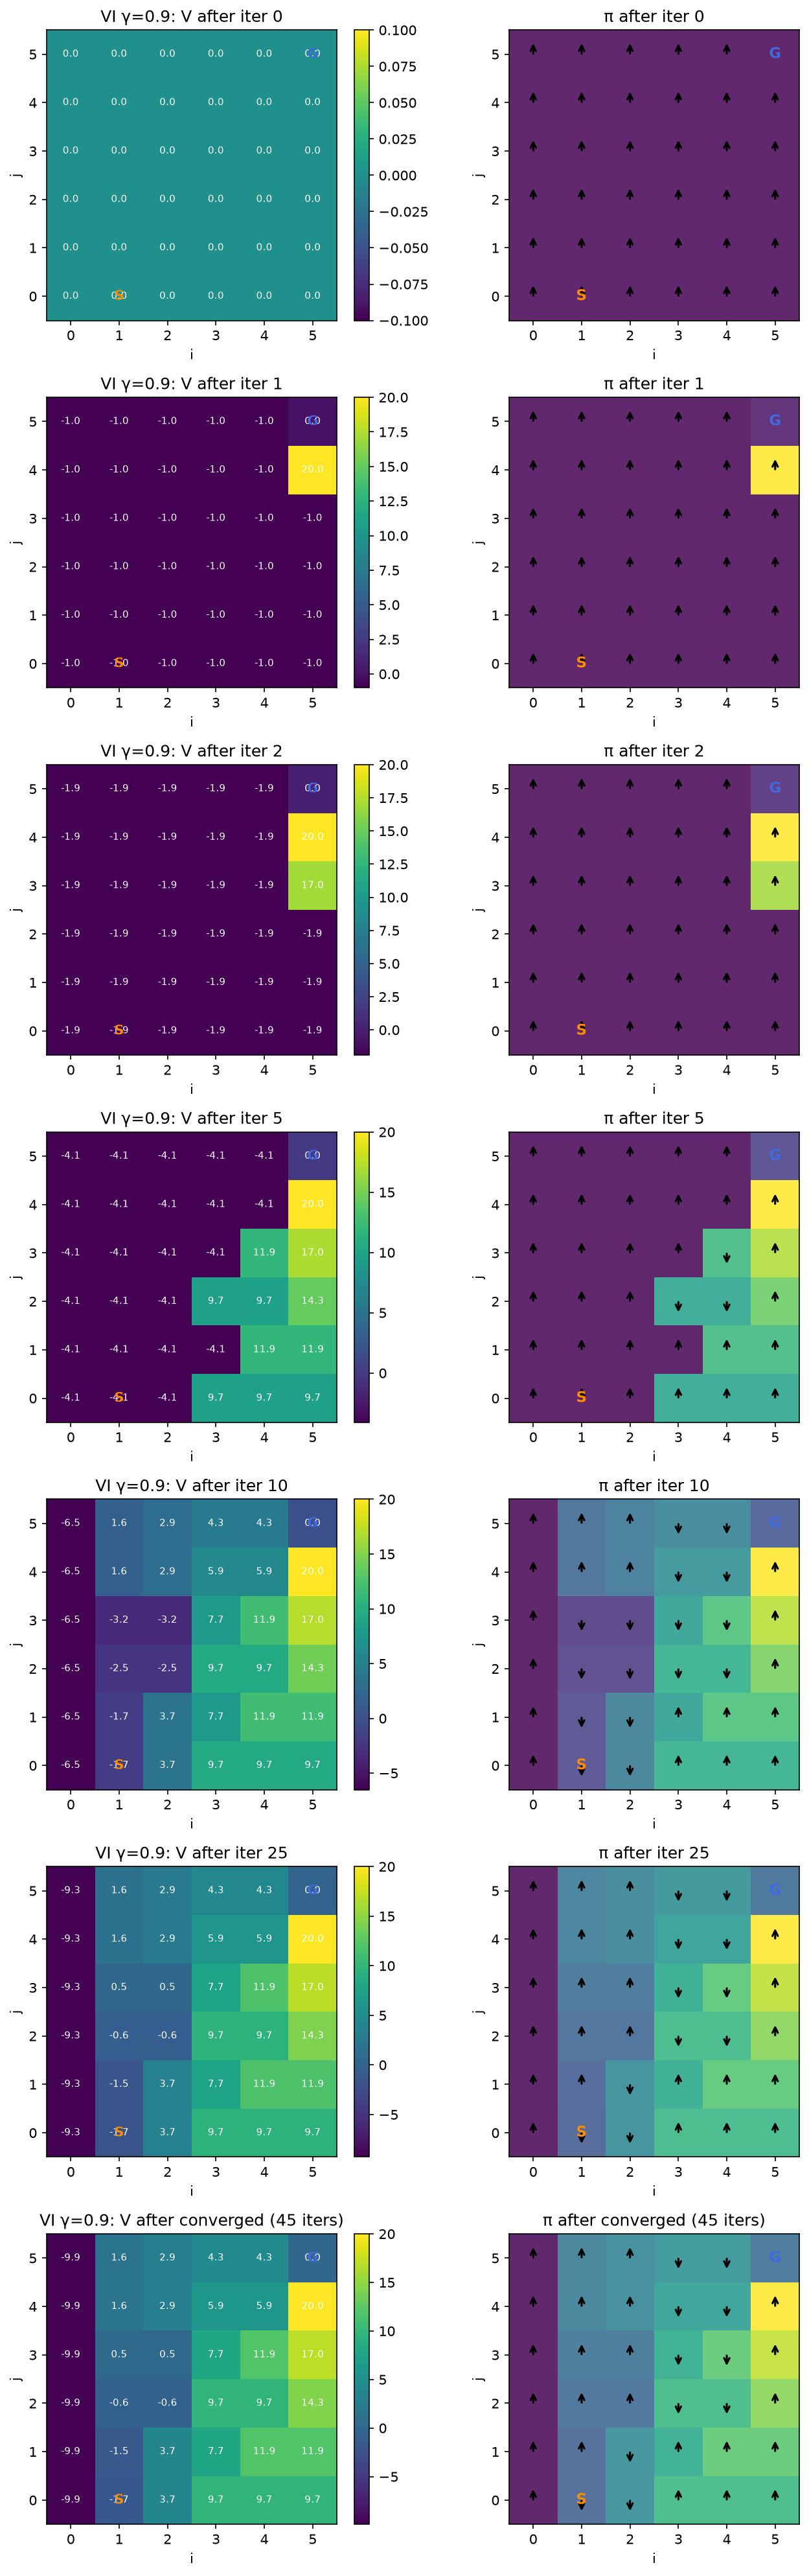
\includegraphics[height=0.82\textheight]{vi_propagation_gamma0.9.png}
\caption{$\gamma=0.9$, starting from $Q=0$: $V$ and greedy $\pi$ after
0, 1, 2, 5, 10, 25 iterations and at convergence (45). Value information
spreads outward from the goal one cell-layer per Bellman update.}
\label{fig:vi-prop}
\end{figure}

\begin{figure}[H]
\centering
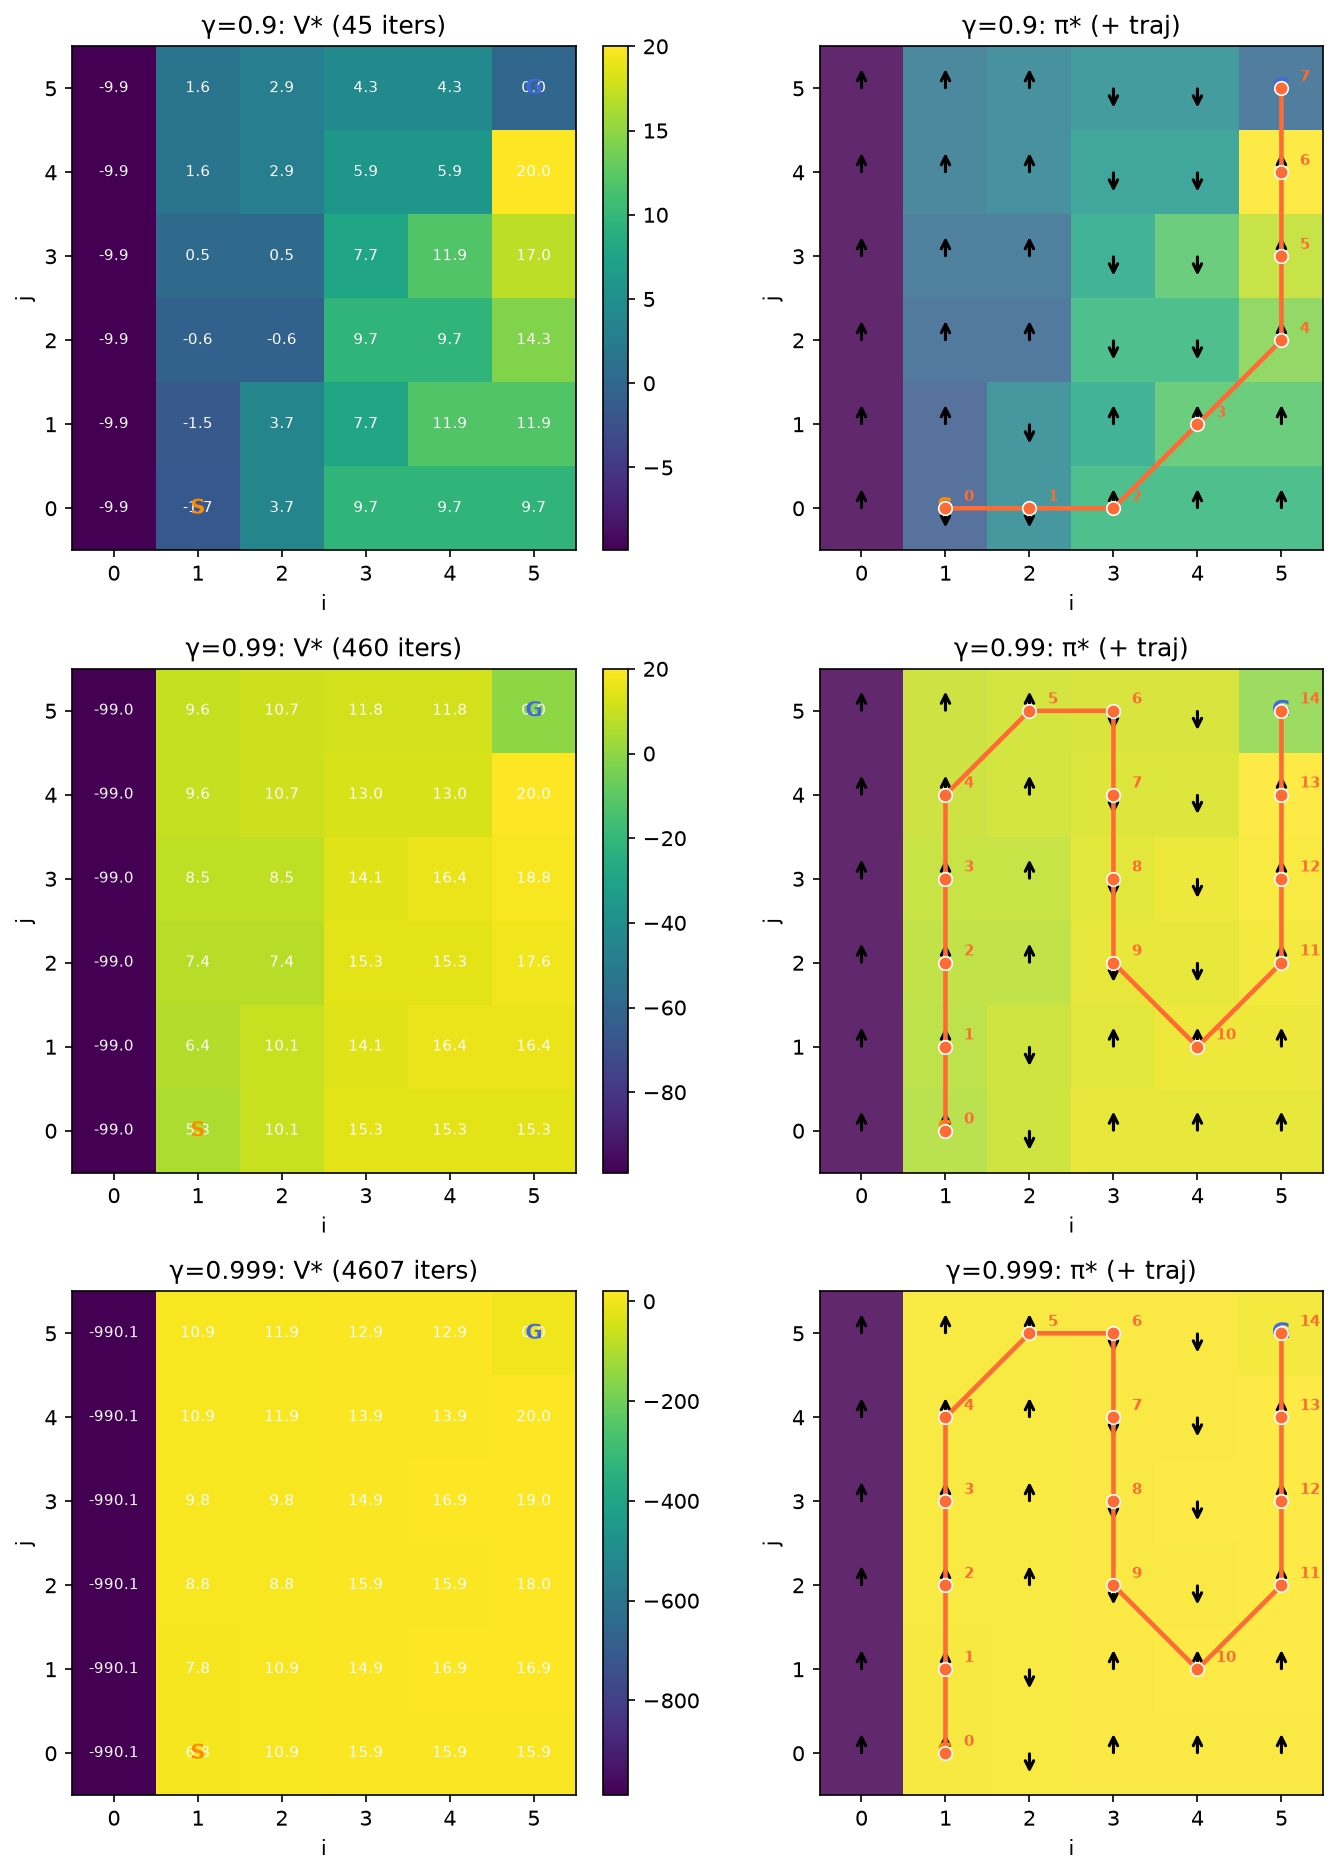
\includegraphics[height=0.82\textheight]{vi_discount_sweep.png}
\caption{Converged $V^*$ and $\pi^*$ (with greedy trajectory) for
$\gamma \in \{0.9, 0.99, 0.999\}$.}
\label{fig:vi-sweep}
\end{figure}

\begin{figure}[H]
\centering
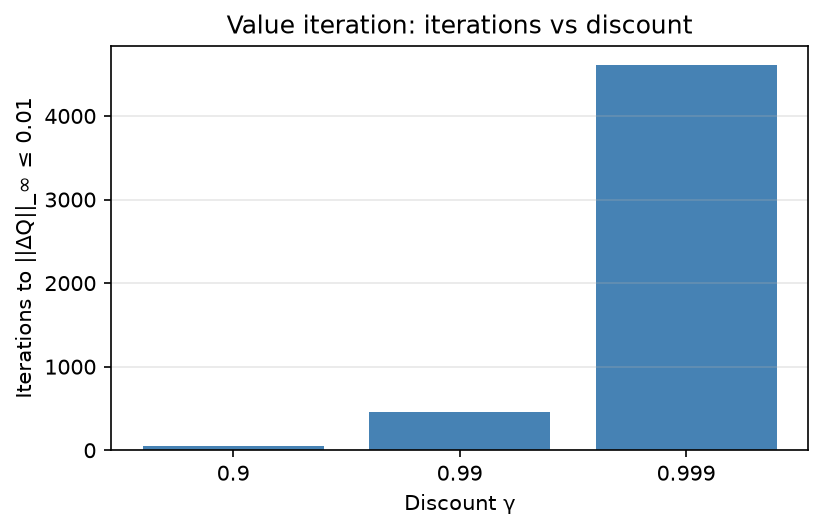
\includegraphics[width=0.7\textwidth]{vi_iterations_vs_discount.png}
\caption{Iterations required to reach the same tolerance versus $\gamma$.}
\label{fig:vi-iters}
\end{figure}

%------------------------------------------------------------------
\section*{6.3 Q-learning}

Settings: $\gamma = 0.9$ (so $\QVI$ is the 45-iteration solution above),
1000 episodes, $\alpha = 0.5$, $Q$ initialised to 0. Only $\epsilon$ is
varied.

\begin{table}[H]
\centering
\begin{tabular}{ccccl}
\toprule
$\epsilon$ & final $E_k = \|Q_k - \QVI\|_\infty$ on $\sreach$ & final $A_k$ & avg return, last 50 ep.\ & greedy route from start \\
\midrule
0   & 14.30 & 95\%  & $7.00$  & safe (not optimal for $\gamma=0.9$) \\
0.1 & 3.11  & 100\% & $4.80$  & risky ($=$ VI) \\
0.5 & 0.00  & 100\% & $-4.82$ & risky ($=$ VI) \\
\bottomrule
\end{tabular}
\end{table}

\begin{figure}[H]
\centering
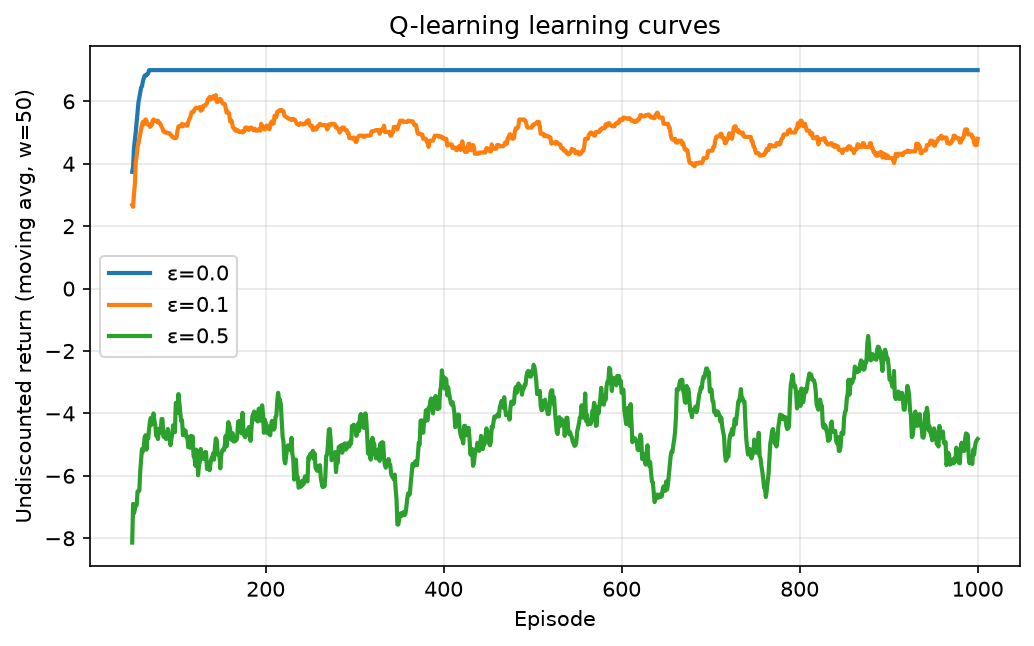
\includegraphics[width=0.75\textwidth]{ql_learning_curves.png}
\caption{Undiscounted return per episode (moving average, window 50)
during training.}
\label{fig:ql-curves}
\end{figure}

\begin{figure}[H]
\centering
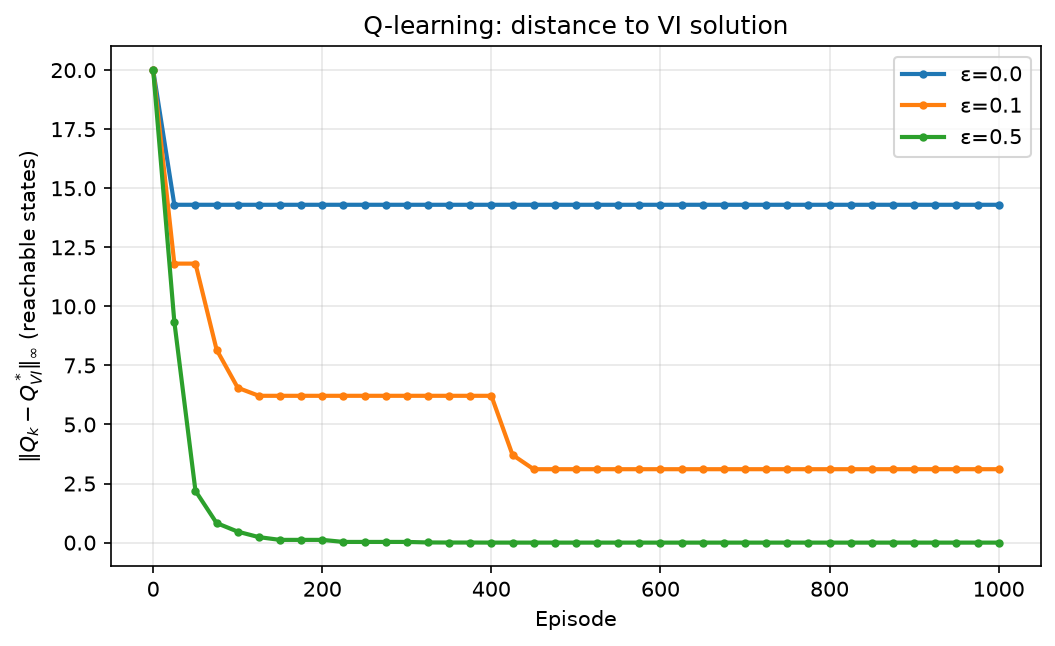
\includegraphics[width=0.75\textwidth]{ql_q_error.png}
\caption{$E_k$, the max-norm distance between the learned $Q$ and $\QVI$
over the reachable states.}
\label{fig:ql-error}
\end{figure}

\begin{figure}[H]
\centering
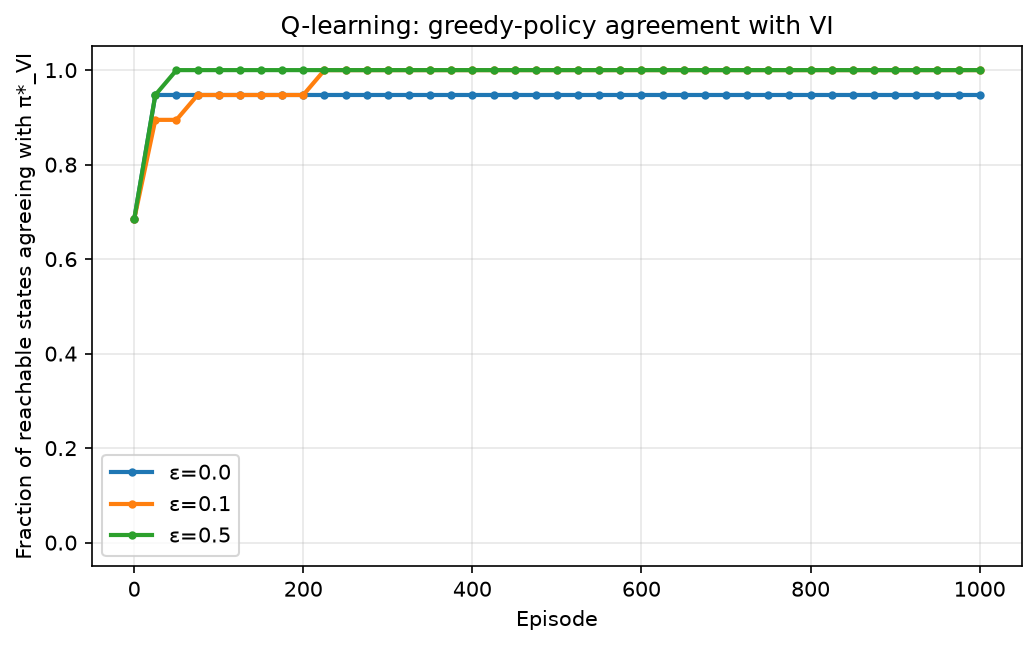
\includegraphics[width=0.75\textwidth]{ql_policy_agreement.png}
\caption{$A_k$, the fraction of reachable non-goal states whose greedy
action matches $\piVI$.}
\label{fig:ql-agree}
\end{figure}

\begin{figure}[H]
\centering
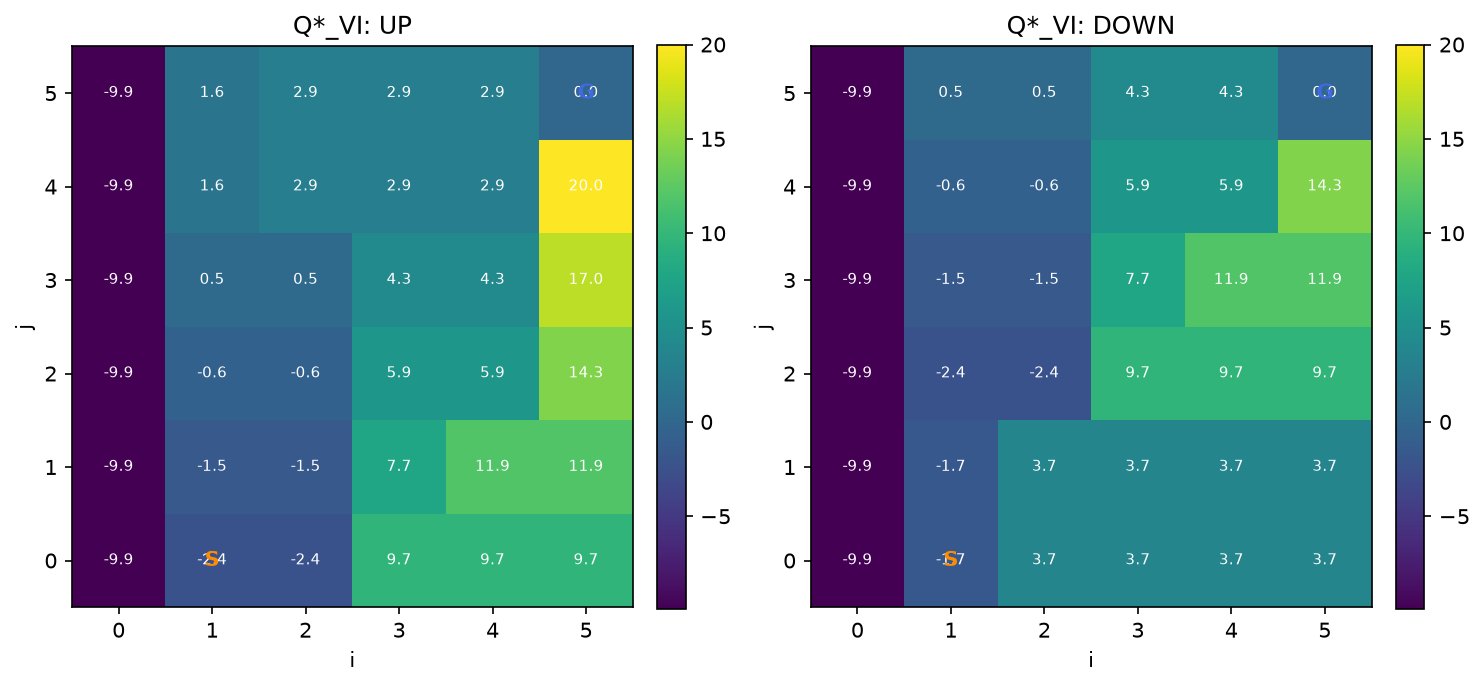
\includegraphics[width=\textwidth]{ql_qstar_vi.png}
\caption{$\QVI$ for $\gamma = 0.9$, the reference the learned Q-functions
are compared to.}
\label{fig:ql-qstar}
\end{figure}

\begin{figure}[H]
\centering
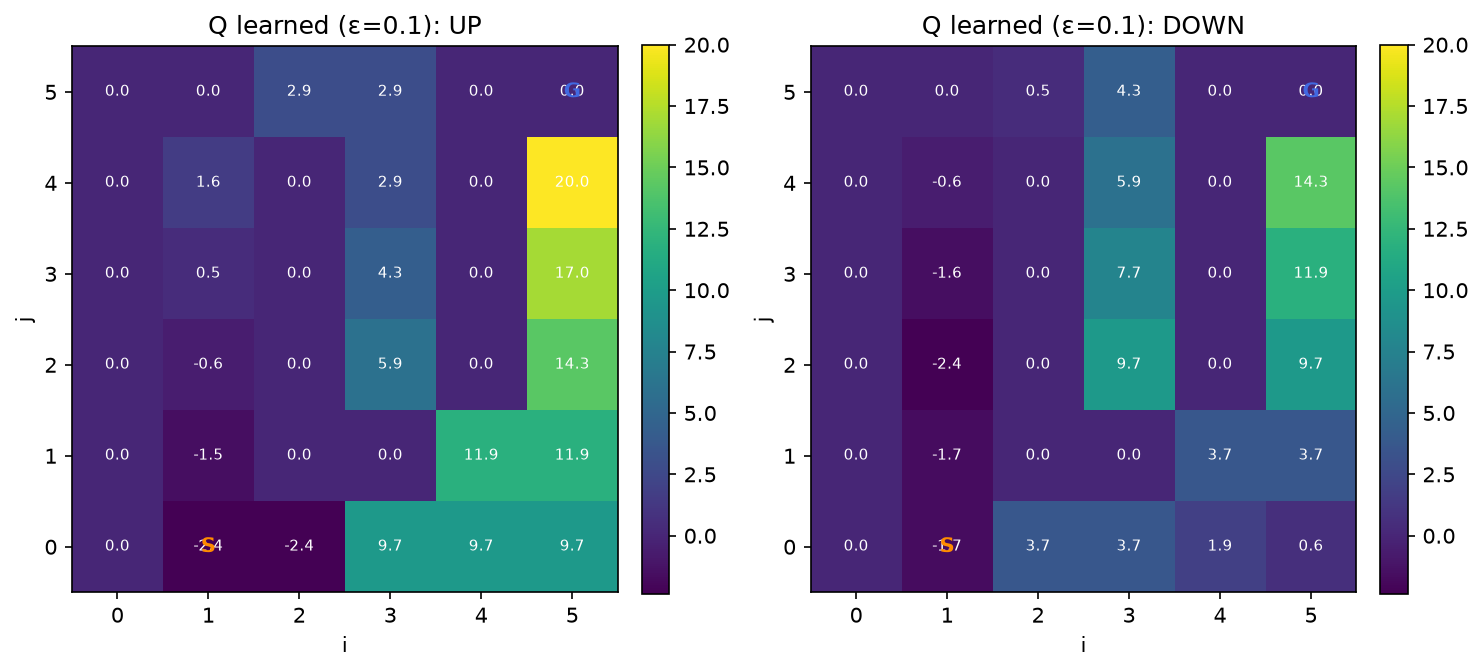
\includegraphics[width=\textwidth]{ql_q_learned_eps0.1.png}
\caption{$Q$ learned with $\epsilon = 0.1$ after 1000 episodes.}
\label{fig:ql-qlearned}
\end{figure}

\begin{figure}[H]
\centering
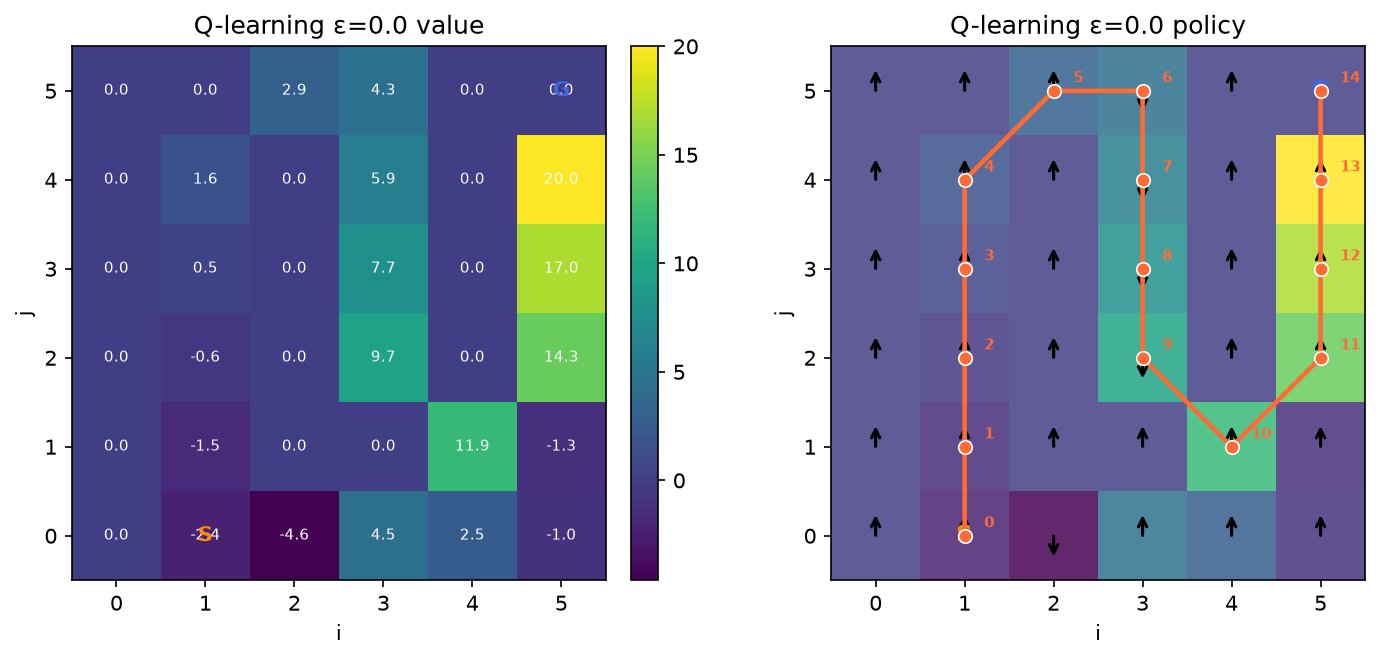
\includegraphics[width=\textwidth]{ql_policy_eps0.0.png}
\caption{Learned greedy policy, $\epsilon = 0$.}
\label{fig:ql-pol0}
\end{figure}

\begin{figure}[H]
\centering
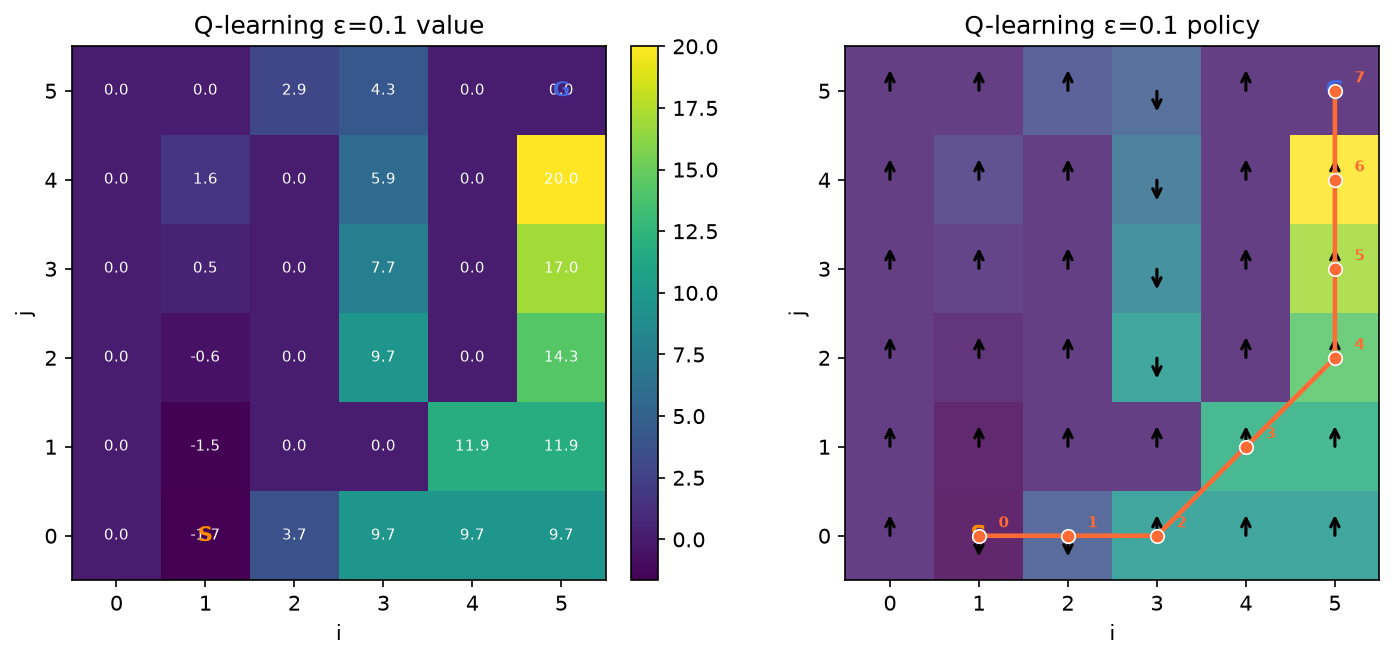
\includegraphics[width=\textwidth]{ql_policy_eps0.1.png}
\caption{Learned greedy policy, $\epsilon = 0.1$.}
\label{fig:ql-pol01}
\end{figure}

\begin{figure}[H]
\centering
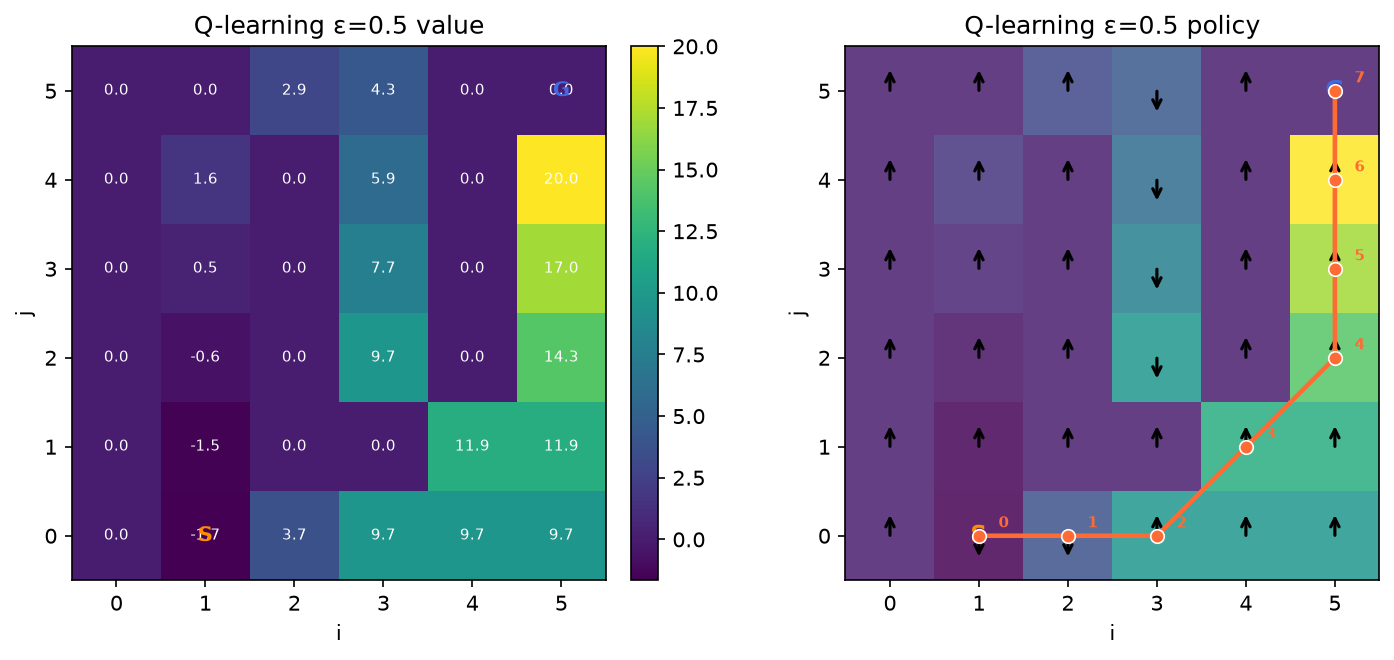
\includegraphics[width=\textwidth]{ql_policy_eps0.5.png}
\caption{Learned greedy policy, $\epsilon = 0.5$.}
\label{fig:ql-pol05}
\end{figure}

%------------------------------------------------------------------
\section*{7. Discussion}

\paragraph{1. Finite horizon and time dependence.}
The shortest path from the start to the goal takes 7 steps, so for
$H \in \{1,3,5\}$ the goal is unreachable from $s_0$ and
$V^*_0(s_0) = -H$ exactly: the balloon pays $-1$ per step no matter what,
and the only thing the policy can still do is avoid the $-5$ cells, which
is why it points UP away from the bottom row. $V^*_0(s_0)$ is therefore
not monotone in $H$. It \emph{falls} ($-1,-3,-5$) while the horizon is too
short, because each extra step is one more forced $-1$, then jumps to $6$
at $H=7$, the first horizon in which the risky route fits. It stays at $6$
for $H=9$ because the goal is absorbing (nothing more is earned after
arrival) and the better safe route needs 14 steps; only at $H=14$ does
$\pi^*_0$ switch to it, giving $V^*_0(s_0) = 7$. Column 0, which can never
reach the goal, keeps falling as $-H$ for every $H$.
Figure~\ref{fig:dp-sweep} shows the same thing spatially: the set of
states with positive value grows outward from the goal by one more layer
per unit of horizon, and everything outside that set is worth $-H$. The
time slices in Figure~\ref{fig:dp-slices} show the same state getting
different actions as time runs out: at $t=0$ (7 steps left) the start
state goes DOWN to begin the risky route, but at $t=1$ (6 left) the goal
can no longer be reached from the start, so $\pi^*_1(s_0) = $ UP to avoid
the penalty cells. When the remaining horizon is too short, the balloon
stops trying to reach the goal and just minimises the cost of the
remaining steps.

\paragraph{2. Discounting and value propagation.}
$\gamma$ sets how far ahead the agent effectively looks. The trapped
column 0 makes this concrete: its exact value is
$-1/(1-\gamma) = -10, -100, -1000$. (VI reports $-9.9, -99.0, -990.1$.
Stopping when the change in $Q$ is below $0.01$ leaves an error of up to
$0.01/(1-\gamma)$ in states whose returns are still accumulating, i.e.\ up
to 10 at $\gamma = 0.999$; near the goal, where the absorbing state pins
values down, the estimates are far more accurate.) $\gamma$ also changes
the optimal policy. The safe route's $+20$ arrives after 13 steps, so it
is worth $20\gamma^{13}$ at the start: about $5.1$ for $\gamma = 0.9$ but
$17.6$ for $\gamma = 0.99$. At $\gamma = 0.9$ the two actions at the start
are worth $Q^*(s_0,\text{DOWN}) = -1.66$ (risky) versus
$Q^*(s_0,\text{UP}) = -2.37$ (safe), so VI takes the $-5$ cells; for
$\gamma \ge 0.99$ the long safe route wins ($5.30$ and $6.82$, approaching
the undiscounted $7$). The number of iterations grows roughly like
$1/(1-\gamma)$: $45, 460, 4607$ (Figure~\ref{fig:vi-iters}). The Bellman
optimality operator is a $\gamma$-contraction, so the error shrinks by a
factor $\gamma$ per sweep and reaching a fixed tolerance takes
$k \approx \log(\mathrm{tol}/\mathrm{err}_0)/\log\gamma \approx
\mathrm{const}/(1-\gamma)$ updates. Figure~\ref{fig:vi-prop} shows the
propagation mechanism: starting from $Q=0$, each update pushes information
about the goal one transition further outward, so after $k$ updates only
states within $k$ steps of the goal have ``seen'' it.

\paragraph{3. Dynamic programming versus value iteration.}
For a long enough horizon the two agree: the DP policy $\pi^*_0$ for
$H=14$ is identical to the VI policy for $\gamma = 0.999$ (both take the
safe route; $V^*_0(s_0) = 7$ versus $V^* = 6.82$), and both share the same
structure everywhere: climb column 5, descend columns 3 and 4 so that the
rightward winds at $(3,1)$ and $(4,2)$ carry the balloon into column 5,
and treat column 0 as a dead end. They need not be identical, for two
reasons. First, the objectives differ: DP maximises an undiscounted sum
over exactly $H$ steps, while VI maximises a discounted infinite sum. The
horizon is a hard cutoff (a route either fits or it does not, which is why
$H=9$ still picks the risky route) while discounting is a soft, geometric
penalty on delay; as $\gamma \to 1$ and $H \to \infty$ these converge, but
for any finite $H$ and $\gamma < 1$ they can rank routes differently.
Second, the DP policy is time-varying, $\pi^*_t$ depends on the remaining
steps, whereas the VI policy is stationary; DP's $\pi^*_0$ happens to
match VI only because at $t=0$ the remaining horizon is large (already at
$t=1$, with 13 steps left, DP's action at the start flips back to DOWN).

\paragraph{4. Value iteration versus Q-learning.}
Value iteration has the model. Its update
\[
Q(s,a) \leftarrow R(s,a) + \gamma \sum_{s'} P(s' \mid s,a)\,
\max_{a'} Q(s',a')
\]
uses the exact reward and the exact next-state distribution, so in one
sweep it can evaluate every $(s,a)$ pair, including states the balloon
would never visit, and it needs no interaction at all. Q-learning only has
\texttt{reset()} and \texttt{step()}. It never sees $P$ or $R$; it sees one
sampled transition $(s_t, a_t, r_t, s_{t+1})$ at a time, and its target
$r_t + \gamma \max_{a'} Q(s_{t+1},a')$ is a single-sample estimate of the
expectation VI computes exactly (the learning rate $\alpha$ averages these
samples over time). Because the sample comes from actually being in $s_t$
and taking $a_t$, Q-learning can only update the pair it just visited. To
learn $Q$ for every state-action pair it therefore has to physically reach
every state and try every action there, which is why it needs many
episodes and an exploratory behaviour policy, and why the handout
evaluates it only on $\sreach$: unvisited rows of the Q-table stay at
their initial value (the untouched cells in
Figures~\ref{fig:ql-pol0}--\ref{fig:ql-pol05} still show the default UP).

\paragraph{5. Exploration in Q-learning.}
More exploration makes the learned $Q$ approach $\QVI$ faster and more
completely, at the cost of worse return while training. With
$\epsilon = 0.5$ every reachable $(s,a)$ pair is tried often, so $A_k$
reaches 100\% within about 50 episodes and $E_k$ is essentially 0 by about
150 (Figures~\ref{fig:ql-error}--\ref{fig:ql-agree}), but half of the
actions are random, so the behaviour return hovers around $-5$
(Figure~\ref{fig:ql-curves}). With $\epsilon = 0.1$ the greedy policy
matches VI after about 220 episodes, but $E_k$ plateaus at $3.1$: the
worst entry is $((5,0),\text{DOWN})$, an action the greedy policy never
takes, so it is updated only on rare random steps (learned $0.6$ versus
$Q^* = 3.7$). The return during training ($\approx 4.8$) is close to the
optimal 6, degraded only by the occasional random step. With
$\epsilon = 0$ the agent is purely greedy, which is not quite the same as
never exploring: because every step costs $-1$, a tried action's estimate
drops below the untried action's initial value of 0, so early on the agent
does wander (its first episode takes 22 steps, and it visits the whole
bottom row). The problem is that an estimate is only refreshed while the
greedy policy keeps choosing that action. The agent tried DOWN at the
start while the bottom-row values were still poor, received a bad sampled
return, and $Q(s_0,\text{DOWN})$ settled at $-7.4$ (its true value is
$-1.66$); from then on UP ($-2.37$) looked better, DOWN was never selected
again, and the stale estimate was never corrected even after the
bottom-row values improved. From about episode 15 onward the agent repeats
the safe route forever: $A_k$ is stuck at 95\% (the start state is the one
disagreement), $E_k$ at $14.3$ ($Q^*((5,4),\text{DOWN}) = 14.3$, but that
pair is never tried, so its entry stays at 0), and the learning curve is a
flat line at 7. That line looks like the best of the three in
Figure~\ref{fig:ql-curves}, but it is the undiscounted return of a policy
that is suboptimal for $\gamma = 0.9$. This is the general problem with
$\epsilon = 0$: without exploration Q-learning has no mechanism to revisit
and correct a pessimistic estimate, so it can converge to the wrong
policy.

\end{document}
